%%%%%%%%%%%%%%%%%%%%%%%%%%%%%%%%%%%%%%%%%%%%%%%%%%%%%%%%%%%%%%%%%
%%  To create image run: (for Windows use imgconvert)
%%
%%  convert -verbose -delay 50 -loop 0 -density 300 -resize 640x480 <name>.pdf <name>.gif
%%
%%%%%%%%%%%%%%%%%%%%%%%%%%%%%%%%%%%%%%%%%%%%%%%%%%%%%%%%%%%%%%%%
%%
%%  Modified from github.com/thetensor-space/Tenscenery
%%
%%%%%%%%%%%%%%%%%%%%%%%%%%%%%%%%%%%%%%%%%%%%%%%%%%%%%%%%%%%%%%%%
\documentclass[beamer,tikz,preview]{standalone}
%\documentclass{beamer}

\setbeamertemplate{navigation symbols}{}
\usefonttheme{professionalfonts} % using non standard fonts for beamer
\usepackage{tikz}
\usepackage{xcolor}
\usepackage{amssymb}
\usepackage{amsmath}

\begin{document}
\begin{frame}
    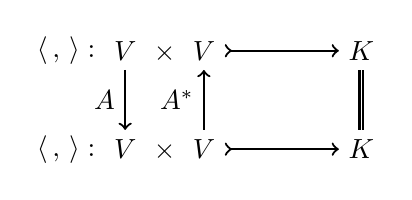
\begin{tikzpicture}
        % Pieces
        \node (GHZ) at (0, 1.25) {$\langle\,,\,\rangle :$};
        \node (W) at (0, 0) {$\langle\,,\,\rangle :$};
        \node (U2) at (0.75, 1.25) {$V$};
        \node (x1) at (1.25, 1.22) {$\times$};
        \node (U1) at (1.75, 1.25) {$V$};
        \node (U0) at (3.75, 1.25) {$K$};
        \node (V2) at (0.75, 0) {$V$};
        \node (x2) at (1.25, -0.03) {$\times$};
        \node (V1) at (1.75, 0) {$V$};
        \node (V0) at (3.75, 0) {$K$};

        % Arrows
        \draw[>->, thick] (U1) -- (U0);
        \draw[>->, thick] (V1) -- (V0);
        \draw[->, thick] (U2) -- (V2) node[midway, left] {$A$};
        \draw[->, thick] (V1) -- (U1) node[midway, left] {$A^*$};
        \draw[-, thick, double] (V0) -- (U0);
    \end{tikzpicture}
\end{frame}

\end{document}